% !TeX root = ../../fheimpl.tex
\documentclass[../../fheimpl.tex]{subfiles}

\begin{document}
	\newif\ifimplismain
	\ifcompileasbook
	\else
	\hypersetup{pageanchor=false}
	\title{Cornami Implementation}
	\implismaintrue
	\maketitle
	\listoffixmes
	\tableofcontents
	\compileasbooktrue
	\hypersetup{pageanchor=true}
	\fi
	
	\section{Cornami Implementation}
	
	\subsection{Composite Scaling}
	Our implementation uses 64-bit words, but we describe the topologies generically so that we can evaluate their performance and cost when using smaller words (composite scaling).
	
	\begin{itemize}
		\item $L$: the number of normal primes in a 64-bit implementation
		\item $k$: the number of special primes in a 64-bit implementation
		\item $m$: the number of cores used to do a single multiplication
		\item $c_L$: the number of \textsf{word}-sized primes needed to hold a normal ``prime''
		\item $c_k$: the number of \textsf{word}-sized primes needed to hold a special ``prime''
		\item $\beta$: the number of partitions in key-switching. Note that this does not change when using composite scaling.
		\item $L^*$: $c_L\cdot L$
		\item $k^*$: $c_k\cdot k$
	\end{itemize}
	
	\subsection{Pre-Extend}
	\begin{figure}[htb]
		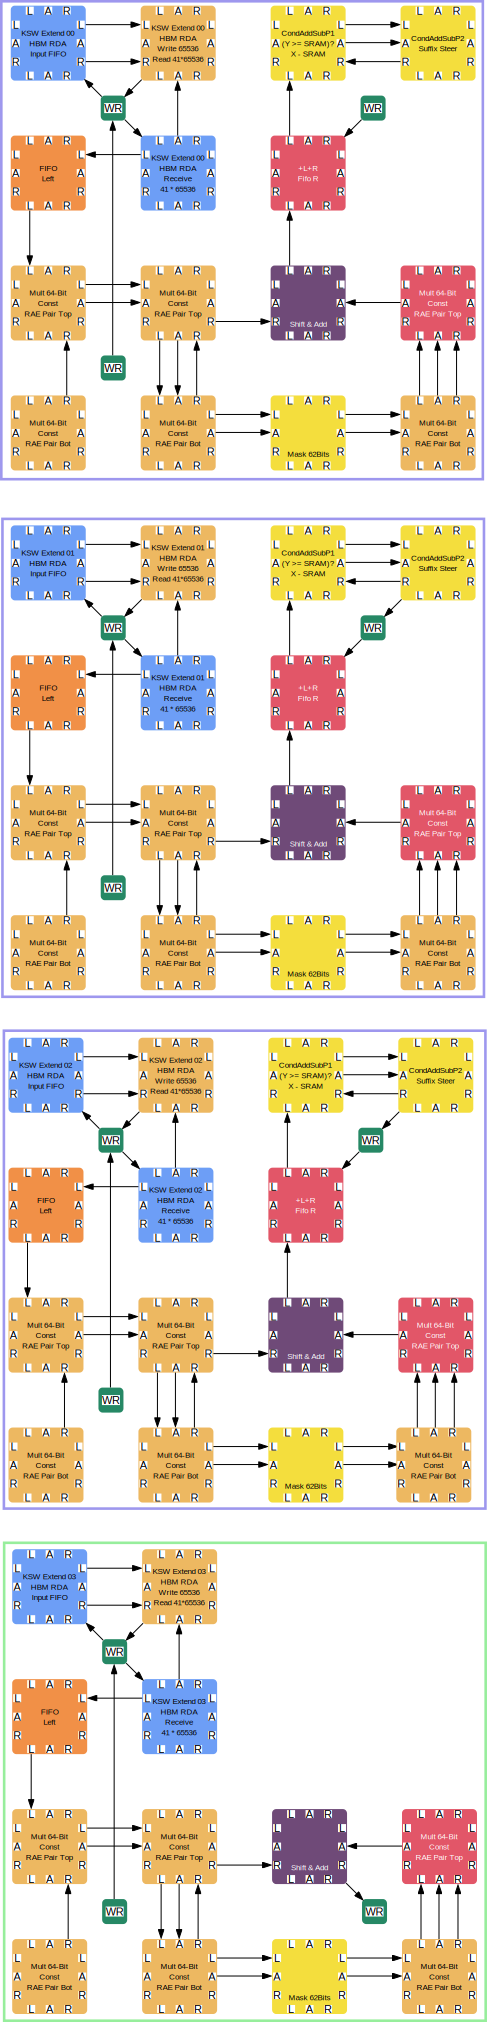
\includegraphics[width=0.45\textwidth,height=8in,keepaspectratio]{graphics/extend.png}
		\caption{Pre-Extend topology for $k=4$}
		\label{fig:preextendtopo}
	\end{figure}
	We use $\beta$ copies of the pre-extend topology, one for each state. Each copy uses
	\[(3m+8)\cdot(c_L\cdot k-1)+(3m+7)\cdot\frac{(c_L\cdot k-1)(c_L\cdot k-2)}{2}\]
	cores, and is used once.
	
	\subsubsection{Improvements}
	While composite scaling can provide advantages, the scaled number of RNS components makes pre-extend in particular much more expensive in terms of cores. Since its \emph{runtime}, on the other hand, is extremely fast (at least an order of magnitude faster than any other step), we would like to avoid the costs associated with composite scaling, even if it costs us time in that step.
	
	The first change is to double the throughput (from four cycles to two cycles) by switching from native 64-bit multiplication to simulated 64-bit multiplication via 32-bit multipliers. While RAE-pair 32-bit multiplication has a throughput of one cycle, 32-bit SCM suffices for our purposes since we're still doing 64-bit multiplication and we can only get 32 bits out per cycle. Each Montgomery multiplication (the bottom eight cores of the green boxes, and the top eight cores of the blue boxes) does three multiplications, only one of which requires the full 128-bit output. For a 96-bit output, we need three 32-bit SCM multiplications, and for the 128-bit output, we need four 32-bit multiplications. Thus the number of cores for multiplication goes from six to ten. The forumula above was designed for the simple case where each multiplication took the same number of cores, but we can substitute in $m=\frac{10}{3}$ for this new design.
	
	At this point, we have doubled the throughput of pre-extend at the cost of a few additional cores. But we need to double the throughput again to get a throughput of one. We do this by doubling the number of tweaked topologies per key-switch state. Now we get two 64-bit outputs every two cycles (per state), giving us an average throughput of one output per clock. Armed with this improvement, we can now describe our hybrid approach to composite scaling. In short, we use regular composite scaling for all \emph{other} keyswitch steps, but we will switch to 64-bit words for pre-extend.
	
	We assume that we are using 27-bit composite scaling parameters, and that the input to keyswitching is $c_L\cdot L$ 27-bit RNS components. The first thing we do is do a CRT recombination on modulus pairs. Given $x_{i,0}\bmod q_{i,0}$ and $x_{i,1} \bmod q_{i,1}$, we can reconstruct $x_i\bmod q_i$ as
	\[(x_{i,0}-x_{i,m1})\cdot (q_{i,1}\cdot (q_{i,1}^{-1}\bmod q_{i,0})) + x_{i,1} \bmod q_i\]
	
	The constant can be pre-computed, which means that (when $c_L=2$) each CRT conversion can be accomplished with one Montgomery addition, one Montgomery subtraction, and one Montgomery multiplication. Using simulated 32-bit arithmetic, this process has a throughput of two cycles, so we need $2$ pre-converters per state to get an average throughput of one cycle for each state. Each converter will be used $k/2$ times.
	
	Similarly, at the end of pre-extend, we need to split the $k$ (for each state) 64-bit components back into $c_L\cdot k$ 27-bit components. We do this using $c_L$ Montgomery reductions, each of which takes 12 cores. These each have a throughput of two cycles, but since we are fixing $c_L=2$ for this approach\footnote{This approach generalizes to $c_L>2$, but the CRT reconstruction becomes more, potentially prohibitively, expensive.}, it suffices to use two post-converters per state.
	
	We can now compare the number of cores in the pure 27-bit composite scaling approach and this ``hybrid'' approach, where we fix $c_L=2$:
	
	In the pure approach, we run $\beta$ copies of the 27-bit pre-extend topology, each on $2k$ RNS components, and each multiply uses a single core. We therefore need
	\[\frac{L}{k}\cdot\parens*{11\cdot(2k-1)+10\cdot\frac{(2k-1)(2k-2)}{2}}\]
	cores.
	
	In the hybrid approach, we run $2\beta$ copies of the 64-bit topology (simulated via 32-bit multiplication), each on $k$ components, plus conversions on both sides. We therefore need
	\[\frac{L}{k}\cdot\parens*{36\cdot(k-1)+34\cdot\frac{(k-1)(k-2)}{2}} + 60\]
	
	These approaches achieve the same throughput and (overall/end-to-end) latency, but pure approach uses 
	\[3kL+7L-60-34\beta\]
	more cores than the hybrid approach.
	
	For the DeSilo-FHE Gold parameters, this 710 cores, or about 10\% of the total.
	
	\subsection{Extend}
	\begin{listing}
		\begin{minted}[frame=single,linenos]{cpp}
void pre_extend(int64_t *c_2, int64_t *pre_extended, std::vector<int> partition,
                std::vector<int64_t> q_product_inverse_mult_r,
                std::vector<std::vector<int64_t>> q_product_mult_r,
                int log_coeff_count) {
  int coeff_count = 1 << log_coeff_count;
	
  const auto q = get_q(log_coeff_count).data();
  const auto q_double = get_q_double(log_coeff_count).data();
  const auto k = get_k(log_coeff_count).data();
	
  auto partition_start_index = partition[0];
  auto partition_start = &c_2[partition_start_index * coeff_count];
  for (auto index = 0; index < partition.size(); index++) {
    std::memcpy(&pre_extended[index * coeff_count], partition_start,
    sizeof(int64_t) * coeff_count);
  }
	
  for (auto index = 0; index < partition.size() - 1; index++) {
    auto offset = (index + 1) * coeff_count;
    auto x = &partition_start[offset];
    auto y = &pre_extended[offset];
    auto depth = partition_start_index + index + 1;
    auto chain_count = 1;
    mont_sub(x, y, y, &q_double[depth], 1, coeff_count);
    mont_enter(y, y, &q_product_inverse_mult_r.data()[index], &q[depth],
    &k[depth], chain_count, coeff_count);
    reduce_2q_to_q(y, y, &q[depth], chain_count, coeff_count);
		
    if (index + 2 < partition.size()) {
      depth += 1;
      chain_count = partition.size() - index - 2;
      auto z = &y[coeff_count];
      mont_enter_tiled_add(y, z, q_product_mult_r[index].data(), &q[depth],
      &k[depth], chain_count, coeff_count);
      reduce_2q_to_q(z, z, &q[depth], chain_count, coeff_count);
    }
  }
}
		\end{minted}
		\caption{Implementation of \textsf{pre\_extend} provided by DESILO on June 10, 2025}
		\label{alg:preextend}
	\end{listing}
	
	\begin{figure}[H]
		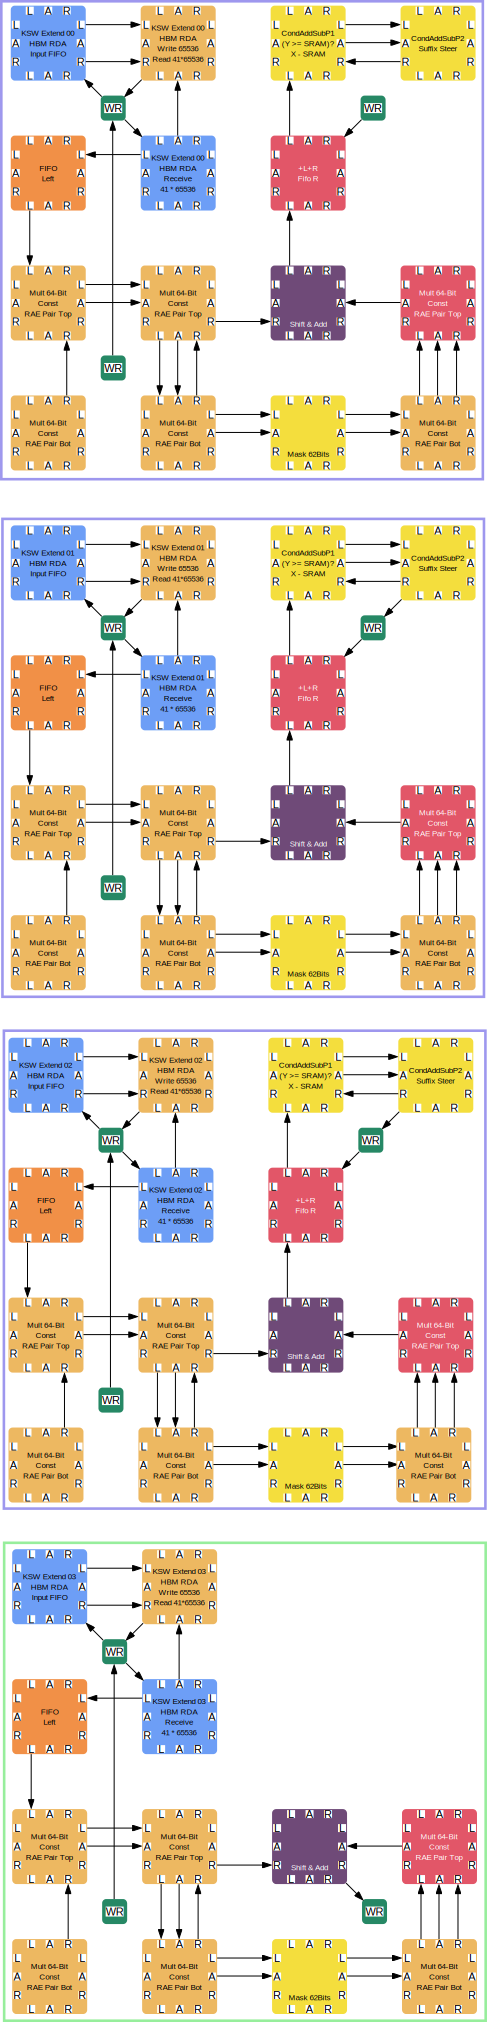
\includegraphics[width=\textwidth,height=8in,keepaspectratio]{graphics/extend.png}
		\caption{Extend topology for $k=4$}
		\label{fig:extendtopo}
	\end{figure}
	
	We use $\beta$ copies of the extend topology, one for each state. Each copy uses
	\[(3m+6)+(9m+6)\cdot(c_L\cdot k-1)\]
	cores, and is used $L^*+k^*$ times.
	
	\subsection{NTT}
	\begin{figure}[H]
		\includegraphics[width=\textwidth,height=\textheight,keepaspectratio]{graphics/ntt.png}
		\caption{NTT topology for $N=2^{16}$}
		\label{fig:ntttopo}
	\end{figure}
	
	Our current NTT topology uses many FIFO cores to assist with data reordering. For small NTTs, we can hold all of the data in a core's SRAM. For larger NTTs, we need FIFOs. The total number of FIFOs needed for an NTT of dimension $N$ with 64-bit words is $\gamma(N)=N/256-4$. Note that if we switch to 32-bit words, each ring element is half the size, meaning that we need to store half as much data. Therefore, the number of FIFOs for 32-bit words is $\gamma(N/2)$, and the number of FIFOs for 16-bit words is $\gamma(N/4)$.
	
	There are $\log_2(N)$ stages, and each stage requires $3m+10$ cores. Therefore, a $N$-dimensional NTT requires $\log_2(N)\cdot(3m+10)+\gamma(N/(64/w))$, where $w$ is the word size in bits. We use $\beta$ copies of the NTT topology, and utilize each one $L^*+k^*$ times.
	
	\subsection{Ring multiplication}
	In this step, we multiply each of the $\beta$ NTT outputs by two key-switch-key components, for a total of $2\beta(L^*+k^*)$ ring products. We use $2\beta$ multiplication topologies, each of size $3m+2$ cores, and use each one $L^*+k^*$ times.
	
	\subsection{Addition}
	This is a fairly complicated step since we are combining $\beta$ (big) ring elements into a single (big) ring element. Since addition requires a single core regardless of word size, the topology size is independent of word size. Each topology requires 54 cores, and adds $\beta$ ring elements together. We use two copies of this topology, and use each copy $L^*+k^*$ times.
	
	\subsection{iNTT}
	Similar to iNTT. The iNTT topology is very similar (but inverted) to the NTT topology. We only use two copies of iNTT, and each one is used $L^*+k^*$ times.
	
	\subsection{ModDown}
	\begin{figure}[h]
		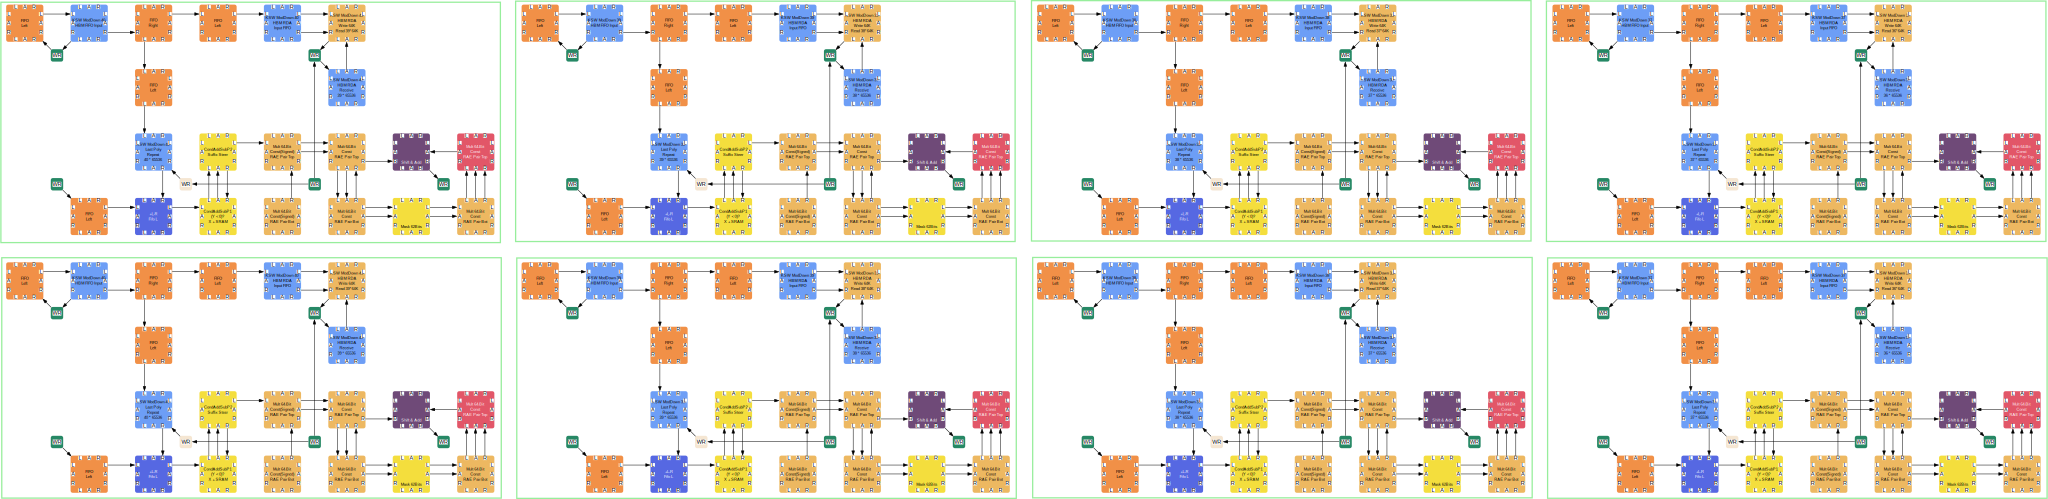
\includegraphics[width=\textwidth,height=\textheight,keepaspectratio]{graphics/moddown.png}
		\caption{ModDown topology for $k=4$}
		\label{fig:moddowntopo}
	\end{figure}
	
	
	
	\ifimplismain
	\else
	\printbibliography
	\fi
	
\end{document}